\documentclass[11pt]{article}
\newcommand{\nombredocumento}{02 · Memoria de cálculo}
% Preámbulo compartido por todos los documentos del proyecto (compilar con pdflatex).
\usepackage[utf8]{inputenc}
\usepackage[T1]{fontenc}
\usepackage{lmodern}
\usepackage{textcomp}
\usepackage[spanish,es-nodecimaldot,es-noshorthands,es-tabla]{babel}
\DeclareUnicodeCharacter{03A9}{\ensuremath{\Omega}}
\DeclareUnicodeCharacter{00B5}{\ensuremath{\mu}}
\DeclareUnicodeCharacter{03BC}{\ensuremath{\mu}}
\DeclareUnicodeCharacter{221A}{\ensuremath{\surd}}
\DeclareUnicodeCharacter{2192}{\ensuremath{\rightarrow}}
\DeclareUnicodeCharacter{2248}{\ensuremath{\approx}}
\DeclareUnicodeCharacter{2212}{\ensuremath{-}}
\DeclareUnicodeCharacter{2264}{\ensuremath{\le}}
\DeclareUnicodeCharacter{2265}{\ensuremath{\ge}}
\DeclareUnicodeCharacter{00D7}{\ensuremath{\times}}
\usepackage[a4paper,top=2.5cm,bottom=2.5cm,left=2.4cm,right=2.4cm,headheight=15pt]{geometry}
\setlength{\emergencystretch}{3em}
\usepackage{amsmath,amssymb,mathtools,bm}
\usepackage{siunitx}
\sisetup{output-decimal-marker={.},group-digits=false,per-mode=symbol,separate-uncertainty}
\usepackage{graphicx,float,booktabs,tabularx,longtable,array,multirow}
\usepackage[font=small,labelfont=bf]{caption}
\usepackage{enumitem}
\setlist{itemsep=2pt,topsep=4pt}
\usepackage[dvipsnames,table]{xcolor}
\usepackage[most]{tcolorbox}
\usepackage{tikz}
\usetikzlibrary{arrows.meta,positioning,shapes.geometric,calc,fit,backgrounds,decorations.markings}
\usepackage[european,straightvoltages]{circuitikz}
\usepackage{listings}
\usepackage{fancyhdr}
\usepackage{titlesec}
\usepackage{xurl}
\usepackage[colorlinks=true,linkcolor=Azul,urlcolor=Azul,citecolor=Azul]{hyperref}

\graphicspath{{../../simulacion/graficas/}{figuras/}}

% ---------------------------------------------------------------- colores
\definecolor{Azul}{HTML}{0D47A1}
\definecolor{Cian}{HTML}{00838F}
\definecolor{Naranja}{HTML}{E65100}
\definecolor{Rojo}{HTML}{C62828}
\definecolor{Verde}{HTML}{2E7D32}
\definecolor{Gris}{HTML}{455A64}
\definecolor{FondoCodigo}{HTML}{F5F7FA}

% ---------------------------------------------------------------- títulos
\titleformat{\section}{\Large\bfseries\color{Azul}}{\thesection}{0.8em}{}
\titleformat{\subsection}{\large\bfseries\color{Cian}}{\thesubsection}{0.8em}{}
\titleformat{\subsubsection}{\normalsize\bfseries\color{Gris}}{\thesubsubsection}{0.8em}{}

% ---------------------------------------------------------------- cabeceras
\pagestyle{fancy}
\fancyhf{}
\fancyhead[L]{\small\color{Gris}\nombredocumento}
\fancyhead[R]{\small\color{Gris}Generador de flujo axial con imanes NdFeB}
\fancyfoot[C]{\small\thepage}
\renewcommand{\headrulewidth}{0.4pt}

% ---------------------------------------------------------------- cajas
\newtcolorbox{nota}[1][Nota]{enhanced,breakable,colback=Azul!4,colframe=Azul!70,
  fonttitle=\bfseries,title={#1},left=6pt,right=6pt}
\newtcolorbox{advertencia}[1][Advertencia]{enhanced,breakable,colback=Rojo!4,colframe=Rojo!80,
  fonttitle=\bfseries,title={#1},left=6pt,right=6pt}
\newtcolorbox{resultado}[1][Resultado]{enhanced,breakable,colback=Verde!5,colframe=Verde!75,
  fonttitle=\bfseries,title={#1},left=6pt,right=6pt}
\newtcolorbox{paso}[1]{enhanced,breakable,colback=white,colframe=Cian!80,
  fonttitle=\bfseries,title={#1},left=6pt,right=6pt}

% ---------------------------------------------------------------- código
\lstdefinestyle{base}{
  basicstyle=\ttfamily\footnotesize,
  backgroundcolor=\color{FondoCodigo},
  frame=single,rulecolor=\color{Gris!40},
  breaklines=true,columns=fullflexible,keepspaces=true,
  keywordstyle=\color{Azul}\bfseries,
  commentstyle=\color{Verde}\itshape,
  stringstyle=\color{Naranja},
  showstringspaces=false,
  extendedchars=true,
  literate={á}{{\'a}}1 {é}{{\'e}}1 {í}{{\'i}}1 {ó}{{\'o}}1 {ú}{{\'u}}1 {ñ}{{\~n}}1
           {Á}{{\'A}}1 {É}{{\'E}}1 {Í}{{\'I}}1 {Ó}{{\'O}}1 {Ú}{{\'U}}1 {Ñ}{{\~N}}1
           {·}{{$\cdot$}}1 {→}{{$\rightarrow$}}1 {Ø}{{\O}}1 {Ω}{{$\Omega$}}1 {µ}{{$\mu$}}1
           {−}{{-}}1 {²}{{$^2$}}1 {√}{{$\surd$}}1 {≈}{{$\approx$}}1
}
\lstdefinestyle{python}{style=base,language=Python}
\lstdefinelanguage{JavaScript}{
  keywords={const,let,var,function,return,class,constructor,new,if,else,for,while,this,true,false,null,typeof,module,export,import},
  sensitive=true,comment=[l]{//},morecomment=[s]{/*}{*/},morestring=[b]',morestring=[b]",morestring=[b]`
}
\lstdefinestyle{js}{style=base,language=JavaScript}
\lstdefinestyle{consola}{style=base,keywordstyle=\color{black}}

% ---------------------------------------------------------------- utilidades
\newcommand{\vect}[1]{\mathbf{#1}}
\newcommand{\unitario}[1]{\mathbf{a}_{#1}}
\newcommand{\dif}{\mathrm{d}}
\DeclareUrlCommand\archivo{\urlstyle{tt}}
\makeatletter
\newcommand{\filasdesde}[1]{\@@input #1 }
\makeatother

\newcommand{\portada}[3]{%
  \begin{titlepage}
    \begin{tikzpicture}[remember picture,overlay]
      \fill[Azul] (current page.north west) rectangle ([yshift=-7cm]current page.north east);
      \node[anchor=north west,text=white,font=\sffamily\bfseries\Huge,text width=16cm,align=left]
        at ([xshift=2.4cm,yshift=-2.2cm]current page.north west) {#1};
      \node[anchor=north west,text=white!85!Azul,font=\sffamily\Large,text width=16cm,align=left]
        at ([xshift=2.4cm,yshift=-4.6cm]current page.north west) {#2};
    \end{tikzpicture}
    \vspace*{7cm}
    \begin{center}
      \begin{tikzpicture}[scale=0.9]
        \foreach \i in {0,...,7} {
          \pgfmathsetmacro{\ang}{45*\i}
          \ifodd\i \def\col{Azul!70}\def\pol{S}\else \def\col{Rojo!80}\def\pol{N}\fi
          \fill[\col] (\ang:2.2) circle (0.55);
          \node[white,font=\bfseries] at (\ang:2.2) {\pol};
        }
        \draw[Gris,line width=1pt] (0,0) circle (3.0);
        \fill[Gris!40] (0,0) circle (0.35);
      \end{tikzpicture}
    \end{center}
    \vfill
    {\large #3\par}
    \vspace{0.6cm}
    {\small\color{Gris}Basado en M.\,N.\,O. Sadiku, \emph{Elementos de Electromagnetismo}, 3.ª ed., Oxford University Press.\par
    Valores numéricos generados por el paquete \texttt{generador\_axial} (\texttt{uv run generador-axial reporte}).\par}
  \end{titlepage}
}

% Archivo generado automáticamente por `generador-axial reporte`. No editar a mano.
\newcommand{\ValGradoIman}{N38}  % Grado comercial del imán
\newcommand{\ValBr}{1.25}  % Remanencia [T]
\newcommand{\ValDiametroIman}{20}  % [mm]
\newcommand{\ValRadioIman}{10.0}  % [mm]
\newcommand{\ValEspesorIman}{5.0}  % [mm]
\newcommand{\ValAreaImanMM}{314.16}  % [mm^2]
\newcommand{\ValPolos}{8}
\newcommand{\ValParesPolos}{4}
\newcommand{\ValPasoPolarGrados}{45.0}  % [grados]
\newcommand{\ValRadioMontaje}{40.0}  % [mm]
\newcommand{\ValBobinas}{8}
\newcommand{\ValEspiras}{180}
\newcommand{\ValEspirasTotales}{1440}
\newcommand{\ValDiametroInteriorBobina}{12.0}  % [mm]
\newcommand{\ValDiametroExteriorBobina}{28.0}  % [mm]
\newcommand{\ValAlturaBobina}{6.0}  % [mm]
\newcommand{\ValEntrehierro}{2.5}  % [mm]
\newcommand{\ValEntrehierroMasAltura}{8.5}  % [mm]
\newcommand{\ValAcoplamiento}{0.85}
\newcommand{\ValCalibreAWG}{26}
\newcommand{\ValDiametroCobre}{0.404}  % [mm]
\newcommand{\ValDiametroEsmaltado}{0.455}  % [mm]
\newcommand{\ValAreaCobreMM}{0.1282}  % [mm^2]
\newcommand{\ValResistividadCobre}{1.72}  % [1e-8 ohm m]
\newcommand{\ValLongitudMediaEspira}{62.83}  % [mm]
\newcommand{\ValLongitudAlambreBobina}{11.31}  % [m]
\newcommand{\ValLongitudAlambreTotal}{90.48}  % [m]
\newcommand{\ValResistenciaBobina}{1.517}  % [ohm]
\newcommand{\ValResistenciaInterna}{12.14}  % [ohm]
\newcommand{\ValVentanaBobinaMM}{48.0}  % [mm^2]
\newcommand{\ValOcupacion}{0.78}
\newcommand{\ValRaizCaraIman}{11.1803}  % sqrt(L^2+R^2) [mm]
\newcommand{\ValTerminoCaraIman}{0.4472}  % L/sqrt(L^2+R^2)
\newcommand{\ValCampoCaraIman}{0.2795}  % [T]
\newcommand{\ValEntrehierroMasEspesor}{7.5}  % g+L [mm]
\newcommand{\ValRaizGL}{12.5000}  % sqrt((g+L)^2+R^2) [mm]
\newcommand{\ValRaizG}{10.3078}  % sqrt(g^2+R^2) [mm]
\newcommand{\ValTerminoUnoG}{0.6000}  % (g+L)/sqrt((g+L)^2+R^2)
\newcommand{\ValTerminoDosG}{0.2425}  % g/sqrt(g^2+R^2)
\newcommand{\ValCampoCaraBobina}{0.2234}  % [T]
\newcommand{\ValEntrehierroAlturaEspesor}{13.5}  % g+h+L [mm]
\newcommand{\ValRaizGHL}{16.8003}  % sqrt((g+h+L)^2+R^2) [mm]
\newcommand{\ValRaizGH}{13.1244}  % sqrt((g+h)^2+R^2) [mm]
\newcommand{\ValPrimitivaEnG}{2.1922}  % F(g) [mm]
\newcommand{\ValPrimitivaEnGH}{3.6759}  % F(g+h) [mm]
\newcommand{\ValDiferenciaPrimitivas}{1.4837}  % F(g+h)-F(g) [mm]
\newcommand{\ValCampoMedioBobina}{0.1545}  % [T]
\newcommand{\ValReduccionPorPromedio}{30.8}  % [%]
\newcommand{\ValFlujoMaximoMicro}{41.270}  % [uWb]
\newcommand{\ValAreaImanM}{3.1416}  % [1e-4 m^2]
\newcommand{\ValCaidaDiodo}{0.30}  % [V]
\newcommand{\ValCaidaPuente}{0.60}  % [V]
\newcommand{\ValCapacitanciaMicro}{220}  % [uF]
\newcommand{\ValTensionNominalCondensador}{50}  % [V]
\newcommand{\ValRpmMaxima}{1200}
\newcommand{\ValTensionDcMaxima}{29.27}  % [V]
\newcommand{\ValMargenCondensador}{41}  % [%]
\newcommand{\ValResistenciaLed}{2200}  % [ohm]
\newcommand{\ValPotenciaNominalResistenciaLed}{0.50}  % [W]
\newcommand{\ValCaidaLed}{2.0}  % [V]
\newcommand{\ValCorrienteLedRefMili}{2.21}  % [mA]
\newcommand{\ValCorrienteLedMaxMili}{12.4}  % [mA]
\newcommand{\ValCorrienteLedLimiteMili}{20}  % [mA]
\newcommand{\ValPotenciaResistenciaLedMax}{0.338}  % [W]
\newcommand{\ValRizadoRef}{251.4}  % [mV]
\newcommand{\ValRpmReferencia}{300}
\newcommand{\ValOmegaMecanicaRef}{31.416}  % [rad/s]
\newcommand{\ValFrecuenciaRef}{20.00}  % [Hz]
\newcommand{\ValPeriodoRefMs}{50.00}  % [ms]
\newcommand{\ValOmegaElectricaRef}{125.66}  % [rad/s]
\newcommand{\ValTensionPicoRef}{7.47}  % [V]
\newcommand{\ValTensionRmsRef}{5.28}  % [V]
\newcommand{\ValTensionDcRef}{6.87}  % [V]
\newcommand{\ValTensionPicoPorBobinaRef}{0.933}  % [V]
\newcommand{\ValRpmCarga}{400}
\newcommand{\ValOmegaMecanicaCarga}{41.89}  % [rad/s]
\newcommand{\ValTensionPicoCarga}{9.96}  % [V]
\newcommand{\ValTensionRmsCarga}{7.04}  % [V]
\newcommand{\ValCorrienteCarga}{0.290}  % [A]
\newcommand{\ValTensionEnCarga}{3.52}  % [V]
\newcommand{\ValPotenciaCarga}{1.021}  % [W]
\newcommand{\ValPotenciaPerdidas}{1.021}  % [W]
\newcommand{\ValPotenciaMecanica}{2.042}  % [W]
\newcommand{\ValParResistenteMili}{48.7}  % [mN m]
\newcommand{\ValEficiencia}{50}  % [%]
\newcommand{\ValBateriaTension}{12}  % [V]
\newcommand{\ValBateriaCapacidad}{7}  % [Ah]
\newcommand{\ValBateriaEnergia}{84}  % [Wh]
\newcommand{\ValBateriaResistencia}{0.05}  % [ohm]
\newcommand{\ValBateriaVacia}{11.8}  % E_oc con SoC = 0 [V]
\newcommand{\ValBateriaLlena}{12.8}  % E_oc con SoC = 1 [V]
\newcommand{\ValBateriaPendiente}{1.0}  % [V]
\newcommand{\ValSocInicial}{50}  % [%]
\newcommand{\ValSocCorte}{20}  % [%]
\newcommand{\ValSocReconexion}{25}  % [%]
\newcommand{\ValTensionOcRef}{12.30}  % [V]
\newcommand{\ValEnergiaUtilRef}{25.2}  % [Wh]
\newcommand{\ValControladorEficiencia}{90}  % [%]
\newcommand{\ValControladorArranque}{3.5}  % [V]
\newcommand{\ValControladorCorrienteMax}{3.0}  % [A]
\newcommand{\ValControladorAbsorcion}{14.4}  % [V]
\newcommand{\ValRpmMicrored}{600}
\newcommand{\ValFemRmsMicrored}{10.56}  % [V]
\newcommand{\ValTensionDcMicrored}{14.34}  % [V]
\newcommand{\ValPotenciaExtraibleMicrored}{2.297}  % [W]
\newcommand{\ValPotenciaHaciaBateria}{2.067}  % [W]
\newcommand{\ValCorrienteCargaMicroredMili}{168}  % [mA]
\newcommand{\ValPotenciaMecanicaMicrored}{4.59}  % [W]
\newcommand{\ValParMicroredMili}{73.1}  % [mN m]
\newcommand{\ValHorasRecarga}{20.8}  % [h]
\newcommand{\ValInversorTension}{110}  % [V]
\newcommand{\ValInversorPico}{155.6}  % [V]
\newcommand{\ValInversorTensionAlta}{220}  % [V]
\newcommand{\ValInversorPicoAlto}{311.1}  % [V]
\newcommand{\ValInversorFrecuencia}{60}  % [Hz]
\newcommand{\ValInversorNominal}{150}  % [W]
\newcommand{\ValInversorEficiencia}{90}  % [%]
\newcommand{\ValRelacionEspiras}{13.0}  % V_pico,AC / V_bat
\newcommand{\ValPotenciaCargaAc}{15}  % [W]
\newcommand{\ValCorrienteAcMili}{136}  % [mA]
\newcommand{\ValPotenciaEntradaInversor}{16.67}  % [W]
\newcommand{\ValCorrienteInversorBateria}{1.36}  % [A]
\newcommand{\ValPotenciaNetaBateria}{-14.60}  % [W]
\newcommand{\ValAutonomiaHoras}{1.73}  % [h]
\newcommand{\ValAutonomiaParadoHoras}{1.51}  % [h]
\newcommand{\ValRpmEquilibrio}{1704}
\newcommand{\ValPotenciaCargaReducida}{5}  % [W]
\newcommand{\ValRpmEquilibrioReducida}{984}
\newcommand{\ValInerciaRotor}{2.415}  % [1e-4 kg m^2]
\newcommand{\ValInductanciaBobinaMili}{0.528}  % [mH]
\newcommand{\ValInductanciaTotalMili}{4.22}  % [mH]
\newcommand{\ValFlujoMaximoReal}{0.827}  % phi_max normalizado
\newcommand{\ValPicoDerivadaFlujo}{0.746}
\newcommand{\ValRmsDerivadaFlujo}{0.559}
\newcommand{\ValFactorCresta}{1.335}
\newcommand{\ValFactorMedia}{0.706}
\newcommand{\ValRelacionFemRealIdeal}{0.930}
\newcommand{\ValPuntosRadiales}{32}
\newcommand{\ValMuestrasPerfil}{256}
\newcommand{\ValPasoIntegracionMili}{5}  % [ms]
\newcommand{\ValParCoulombMili}{3.0}  % [mN m]
\newcommand{\ValCoefViscosoMicro}{15.0}  % [uN m s]
\newcommand{\ValCoefVentilacionNano}{15.0}  % [nN m s^2]
\newcommand{\ValParMaximoMotriz}{0.30}  % [N m]
\newcommand{\ValVelocidadVacioMotriz}{1500}  % [RPM]
\newcommand{\ValParImpulso}{0.08}  % [N m]
\newcommand{\ValDuracionImpulso}{0.5}  % [s]
\newcommand{\ValCapacidadTermica}{100}  % [J/K]
\newcommand{\ValConveccionNatural}{8}  % [W/m^2K]
\newcommand{\ValConveccionForzada}{0.15}  % [W/m^2K por rad/s]
\newcommand{\ValCoefCobre}{0.393}  % [%/K]
\newcommand{\ValCoefRemanencia}{-0.12}  % [%/K]
\newcommand{\ValTemperaturaMaximaPla}{55}  % [C]
\newcommand{\ValBateriaRCero}{25}  % [mohm]
\newcommand{\ValBateriaRPolarizacion}{30}  % [mohm]
\newcommand{\ValBateriaTau}{30}  % [s]
\newcommand{\ValBateriaPeukert}{1.12}
\newcommand{\ValBateriaEtaCoulomb}{95}  % [%]
\newcommand{\ValBateriaEtaLlena}{60}  % [%]
\newcommand{\ValBateriaSocGas}{85}  % [%]
\newcommand{\ValBateriaAutodescarga}{3}  % [%/mes]
\newcommand{\ValBateriaSocFlotacion}{99.5}  % [%]
\newcommand{\ValBateriaFactorGas}{1500}
\newcommand{\ValBateriaPendienteGas}{50}
\newcommand{\ValControladorFlotacion}{13.8}  % [V]
\newcommand{\ValConsumoControladorMili}{8}  % [mA]
\newcommand{\ValInversorVacio}{3.6}  % [W]
\newcommand{\ValInversorCoefCuadratico}{5.81}  % [1e-4 1/W]
\newcommand{\ValInversorCorte}{10.8}  % [V]
\newcommand{\ValInversorReconexion}{12.3}  % [V]
\newcommand{\ValParReferencia}{0.07}  % [N m]
\newcommand{\ValRpmRegimenRef}{483}
\newcommand{\ValPotenciaEjeRef}{2.40}  % [W]
\newcommand{\ValPotenciaElectromagneticaRef}{2.21}  % [W]
\newcommand{\ValPerdidasCobreRef}{0.986}  % [W]
\newcommand{\ValPerdidasRozamientoRef}{0.192}  % [W]
\newcommand{\ValPerdidasFoucaultMili}{1.65}  % [mW]
\newcommand{\ValPotenciaBateriaRef}{0.96}  % [W]
\newcommand{\ValEficienciaRef}{40}  % [%]
\newcommand{\ValTensionDcRefReal}{3.50}  % [V]
\newcommand{\ValCorrienteGeneradorRef}{0.281}  % [A]
\newcommand{\ValTemperaturaRegimenRef}{27.8}  % [C]
\newcommand{\ValRpmConCargaRef}{483}
\newcommand{\ValPotenciaEntradaInversorRef}{18.7}  % [W]
\newcommand{\ValCorrienteNetaConCarga}{-1.48}  % [A]
\newcommand{\ValRpmParMaximo}{1002}
\newcommand{\ValPotenciaBateriaParMaximo}{4.35}  % [W]
\newcommand{\ValRizadoBajo}{18.8}  % [V] con 220 uF
\newcommand{\ValRizadoAlto}{0.88}  % [V] con 4700 uF
\newcommand{\ValRpmPicoImpulso}{505}
\newcommand{\ValTiempoParadaImpulso}{2.7}  % [s]
\newcommand{\ValHorasHastaAbsorcion}{4.0}  % [h]
\newcommand{\ValHorasHastaFlotacion}{8.2}  % [h]
\newcommand{\ValCorrienteFlotacionMili}{21}  % [mA]



\begin{document}

\portada{Memoria de cálculo}
        {Cálculo numérico paso a paso del prototipo: campo, flujo, tensión, resistencia, potencia y par}
        {Documento 2 de 5 · Resultados del modelo analítico}

\tableofcontents
\newpage

%=====================================================================
\section{Cómo se obtuvo cada número}
%=====================================================================
Todos los valores de este documento se escriben a partir del archivo
\archivo{docs/latex/generado/valores.tex}, que genera automáticamente el comando
\begin{lstlisting}[style=consola]
uv run generador-axial reporte
\end{lstlisting}
a partir del diseño definido en \archivo{src/generador_axial/configuracion.py}. Si se cambia un parámetro del
diseño (por ejemplo, el número de espiras) y se recompilan los PDF con \archivo{docs/compilar_pdf.sh}, todas las
cifras de este documento se actualizan solas. Así se evita que la documentación y el código digan cosas distintas.

Cada paso sigue la misma estructura: \textbf{fórmula} (deducida en el Documento~1) $\rightarrow$
\textbf{sustitución} de los datos $\rightarrow$ \textbf{resultado}.

%=====================================================================
\section{Datos de entrada}
%=====================================================================
\begin{table}[H]
\centering
\caption{Parámetros del diseño.}
\begin{tabular}{llr}
\toprule
Símbolo & Descripción & Valor\\
\midrule
$B_r$ & Remanencia del imán (grado \ValGradoIman) & \ValBr\ T\\
$R$ & Radio del imán ($\varnothing$\,\ValDiametroIman\ mm) & \ValRadioIman\ mm\\
$L$ & Espesor del imán & \ValEspesorIman\ mm\\
$P$ & Número de polos & \ValPolos\\
$r_m$ & Radio de montaje de imanes y bobinas & \ValRadioMontaje\ mm\\
$N_b$ & Número de bobinas & \ValBobinas\\
$N$ & Espiras por bobina & \ValEspiras\\
$D_i,\ D_e$ & Diámetros interior y exterior de la bobina & \ValDiametroInteriorBobina\ / \ValDiametroExteriorBobina\ mm\\
$h$ & Altura (espesor axial) de la bobina & \ValAlturaBobina\ mm\\
$g$ & Entrehierro (cara del imán a cara de la bobina) & \ValEntrehierro\ mm\\
$k$ & Factor de acoplamiento & \ValAcoplamiento\\
AWG & Calibre del alambre (cobre $\varnothing$\,\ValDiametroCobre\ mm, esmaltado $\varnothing$\,\ValDiametroEsmaltado\ mm) & \ValCalibreAWG\\
$\rho_{Cu}$ & Resistividad del cobre a \SI{20}{\celsius} & \ValResistividadCobre$\times10^{-8}$\ $\Omega\cdot$m\\
$V_D$ & Caída por diodo (Schottky) & \ValCaidaDiodo\ V\\
$C$ & Condensador de filtro & \ValCapacitanciaMicro\ $\mu$F / \ValTensionNominalCondensador\ V\\
$R_{LED}$ & Resistencia limitadora del LED & \ValResistenciaLed\ $\Omega$, \ValPotenciaNominalResistenciaLed\ W\\
\bottomrule
\end{tabular}
\end{table}

%=====================================================================
\section{Campo magnético}
%=====================================================================

\begin{paso}{Paso 1 · Área de la cara del imán}
\[
  A_{im}=\pi R^2=\pi\,(\ValRadioIman\ \text{mm})^2=\ValAreaImanMM\ \text{mm}^2=\ValAreaImanM\times10^{-4}\ \text{m}^2 .
\]
\end{paso}

\begin{paso}{Paso 2 · Campo en la cara del imán ($z=0$)}
Con $z=0$ el segundo término de la fórmula del campo se anula:
\[
  B_z(0)=\frac{B_r}{2}\,\frac{L}{\sqrt{L^2+R^2}}
  =\frac{\ValBr}{2}\cdot\frac{\ValEspesorIman}{\ValRaizCaraIman}
  =\frac{\ValBr}{2}\cdot\ValTerminoCaraIman
  =\boxed{\ValCampoCaraIman\ \text{T}}
\]
(Las longitudes pueden ir en mm porque aparecen como cociente.)
\end{paso}

\begin{paso}{Paso 3 · Campo en la cara de la bobina ($z=g=\ValEntrehierro$ mm)}
\begin{align*}
  \frac{g+L}{\sqrt{(g+L)^2+R^2}}&=\frac{\ValEntrehierroMasEspesor}{\ValRaizGL}=\ValTerminoUnoG,\\
  \frac{g}{\sqrt{g^2+R^2}}&=\frac{\ValEntrehierro}{\ValRaizG}=\ValTerminoDosG,\\
  B_z(g)&=\frac{\ValBr}{2}\left(\ValTerminoUnoG-\ValTerminoDosG\right)=\boxed{\ValCampoCaraBobina\ \text{T}}
\end{align*}
\end{paso}

\begin{paso}{Paso 4 · Campo medio en el espesor de la bobina ($g\le z\le g+h$)}
Con $F(z)=\sqrt{(z+L)^2+R^2}-\sqrt{z^2+R^2}$ (en mm):
\begin{align*}
  F(g)&=\sqrt{(\ValEntrehierroMasEspesor)^2+\ValRadioIman^2}-\sqrt{\ValEntrehierro^2+\ValRadioIman^2}
       =\ValRaizGL-\ValRaizG=\ValPrimitivaEnG,\\
  F(g+h)&=\sqrt{(\ValEntrehierroAlturaEspesor)^2+\ValRadioIman^2}-\sqrt{\ValEntrehierroMasAltura^2+\ValRadioIman^2}
       =\ValRaizGHL-\ValRaizGH=\ValPrimitivaEnGH,\\
  \bar B_z&=\frac{B_r}{2h}\big[F(g+h)-F(g)\big]=\frac{\ValBr}{2\cdot\ValAlturaBobina}\cdot\ValDiferenciaPrimitivas
          =\boxed{\ValCampoMedioBobina\ \text{T}}
\end{align*}
El campo medio es un \ValReduccionPorPromedio\,\% menor que el campo en la cara de la bobina.
\end{paso}

\begin{figure}[H]
\centering
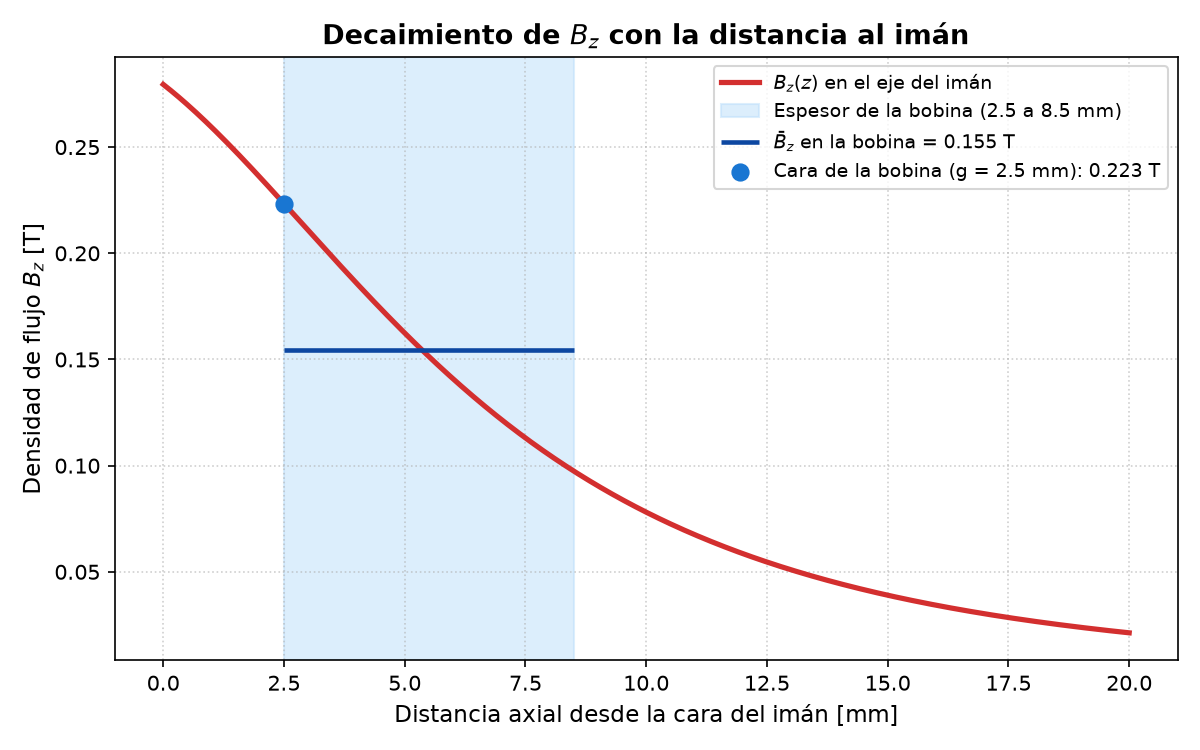
\includegraphics[width=0.85\linewidth]{01_campo_magnetico_vs_distancia.png}
\caption{Campo axial $B_z(z)$. La franja azul es el volumen ocupado por las espiras; la línea horizontal es el
promedio $\bar B_z$ que se usa en el cálculo del flujo.}
\end{figure}

%=====================================================================
\section{Flujo magnético}
%=====================================================================
\begin{paso}{Paso 5 · Flujo máximo por espira}
\[
  \Phi_{max}=k\,\bar B_z\,A_{im}=\ValAcoplamiento\times\ValCampoMedioBobina\ \text{T}\times\ValAreaImanM\times10^{-4}\ \text{m}^2
  =\boxed{\ValFlujoMaximoMicro\ \mu\text{Wb}}
\]
\end{paso}

%=====================================================================
\section{Cinemática a \ValRpmReferencia\ RPM (velocidad de referencia)}
%=====================================================================
\begin{paso}{Paso 6 · Velocidades y frecuencia}
\begin{align*}
  \omega_m&=\frac{2\pi\cdot\text{RPM}}{60}=\frac{2\pi\cdot\ValRpmReferencia}{60}=\ValOmegaMecanicaRef\ \text{rad/s},\\
  f_e&=\frac{P\cdot\text{RPM}}{120}=\frac{\ValPolos\cdot\ValRpmReferencia}{120}=\boxed{\ValFrecuenciaRef\ \text{Hz}},\\
  \omega_e&=2\pi f_e=\frac{P}{2}\,\omega_m=\ValOmegaElectricaRef\ \text{rad/s},\qquad
  T_e=\frac{1}{f_e}=\ValPeriodoRefMs\ \text{ms}.
\end{align*}
\end{paso}

%=====================================================================
\section{Tensión inducida}
%=====================================================================
\begin{paso}{Paso 7 · Fem pico, eficaz y rectificada a \ValRpmReferencia\ RPM}
\begin{align*}
  N_{total}&=N_b\cdot N=\ValBobinas\times\ValEspiras=\ValEspirasTotales,\\
  V_{pico}&=N_{total}\,\omega_e\,\Phi_{max}=\ValEspirasTotales\times\ValOmegaElectricaRef\times\ValFlujoMaximoMicro\times10^{-6}
          =\boxed{\ValTensionPicoRef\ \text{V}},\\
  V_{pico,\,bobina}&=V_{pico}/N_b=\ValTensionPicoPorBobinaRef\ \text{V},\\
  V_{RMS}&=\frac{V_{pico}}{\sqrt2}=\frac{\ValTensionPicoRef}{1.4142}=\boxed{\ValTensionRmsRef\ \text{V}},\\
  V_{DC}&\approx V_{pico}-2V_D=\ValTensionPicoRef-\ValCaidaPuente=\boxed{\ValTensionDcRef\ \text{V}}.
\end{align*}
\end{paso}

\begin{figure}[H]
\centering
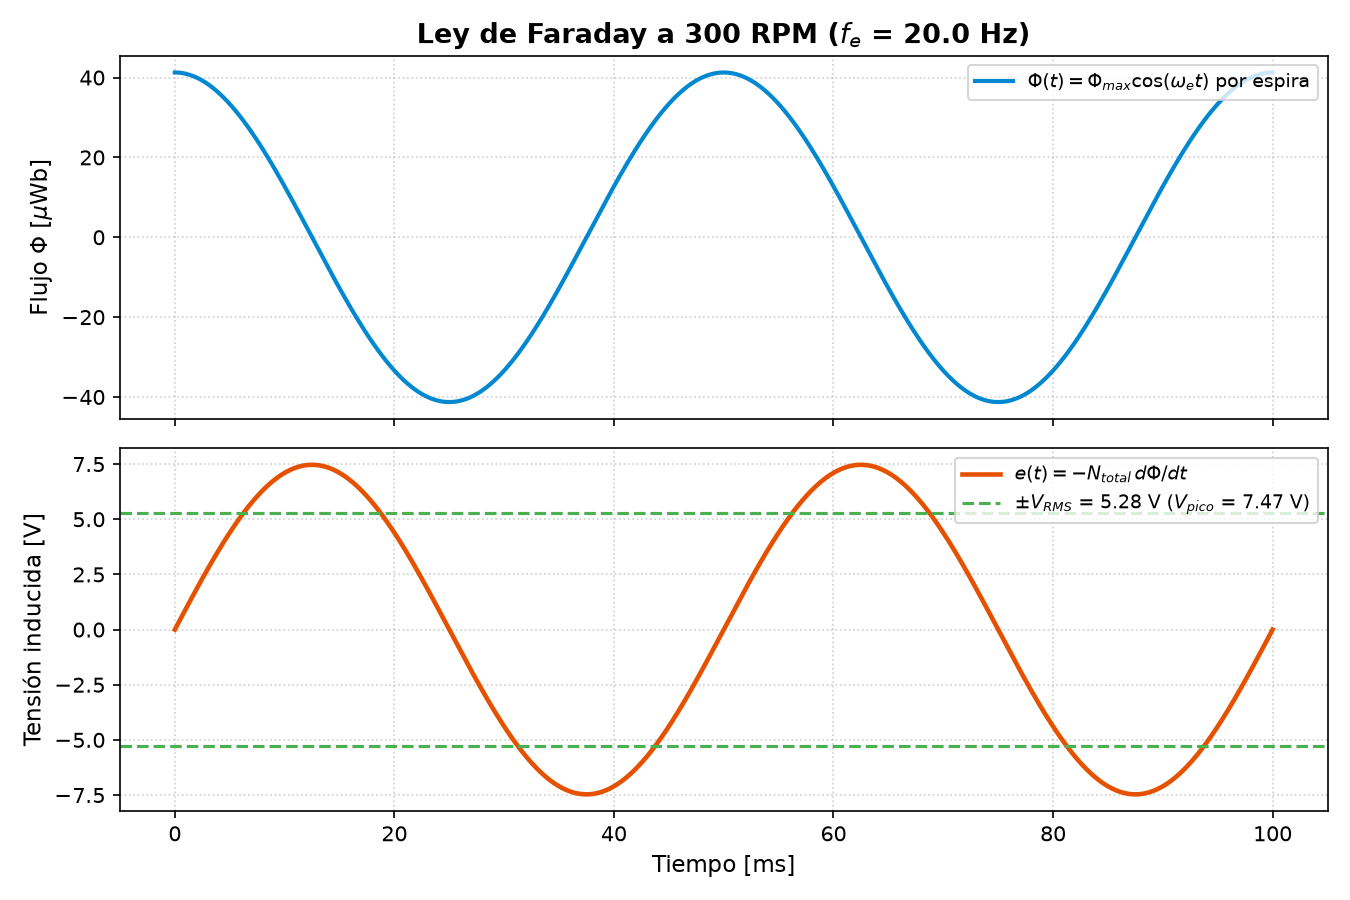
\includegraphics[width=0.85\linewidth]{02_flujo_y_voltaje_inducido_faraday.png}
\caption{Flujo por espira $\Phi(t)$ y fem total $e(t)=-N_{total}\,\dif\Phi/\dif t$ a \ValRpmReferencia\ RPM. La fem
es máxima cuando el flujo pasa por cero (máxima pendiente) y nula cuando el flujo es máximo.}
\end{figure}

\begin{figure}[H]
\centering
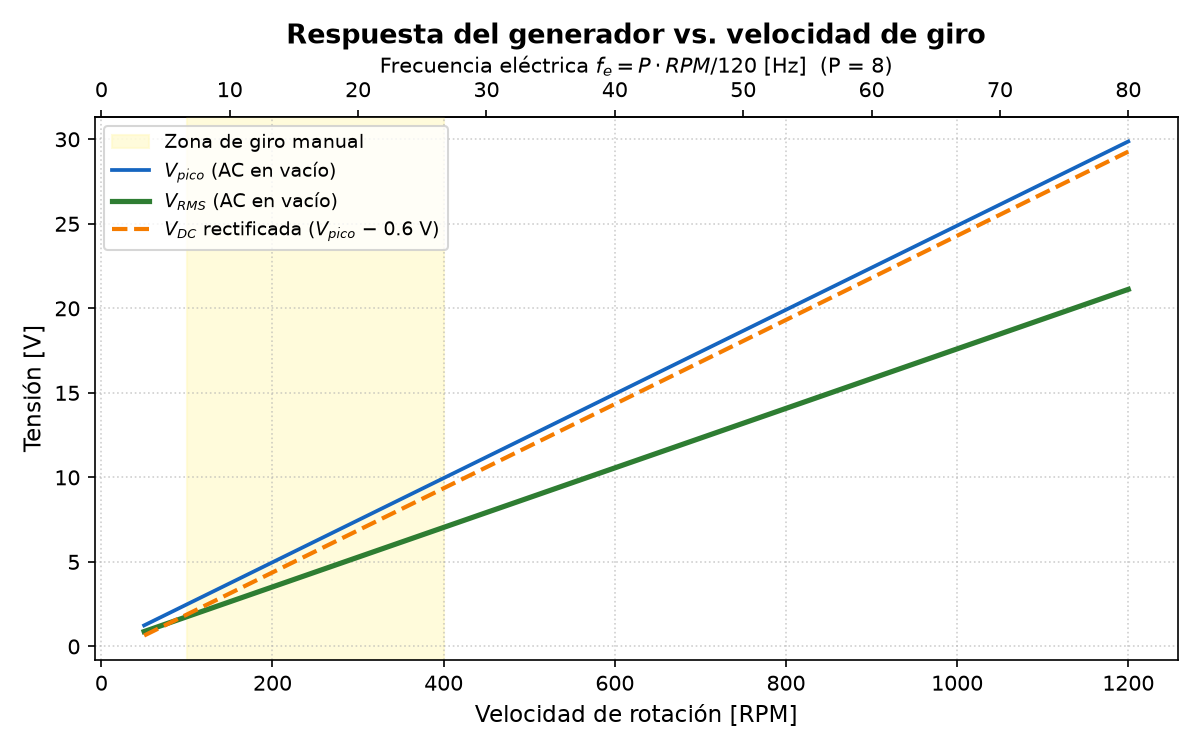
\includegraphics[width=0.85\linewidth]{03_voltaje_rms_vs_rpm.png}
\caption{Las tensiones crecen linealmente con la velocidad porque $V_{pico}\propto\omega_e\propto\text{RPM}$. El eje
superior muestra la frecuencia eléctrica correspondiente.}
\end{figure}

%=====================================================================
\section{Resistencia interna y ocupación de la bobina}
%=====================================================================
\begin{paso}{Paso 8 · Longitud de alambre}
\begin{align*}
  \ell_m&=\pi\,\frac{D_i+D_e}{2}=\pi\,\frac{\ValDiametroInteriorBobina+\ValDiametroExteriorBobina}{2}=\ValLongitudMediaEspira\ \text{mm},\\
  L_{bobina}&=N\,\ell_m=\ValEspiras\times\ValLongitudMediaEspira\ \text{mm}=\ValLongitudAlambreBobina\ \text{m},\\
  L_{total}&=N_b\,L_{bobina}=\ValLongitudAlambreTotal\ \text{m}.
\end{align*}
\end{paso}

\begin{paso}{Paso 9 · Resistencia}
\begin{align*}
  A_{Cu}&=\frac{\pi d^2}{4}=\frac{\pi\,(\ValDiametroCobre)^2}{4}=\ValAreaCobreMM\ \text{mm}^2,\\
  R_{bobina}&=\rho_{Cu}\,\frac{L_{bobina}}{A_{Cu}}=\ValResistenciaBobina\ \Omega,\\
  R_{int}&=N_b\,R_{bobina}=\boxed{\ValResistenciaInterna\ \Omega}.
\end{align*}
Este es el valor que debe medirse con el multímetro entre los terminales de salida (a \SI{20}{\celsius}).
\end{paso}

\begin{paso}{Paso 10 · ¿Caben las espiras? (factor de ocupación)}
La ventana de bobinado mide $\frac{D_e-D_i}{2}\times h=\ValVentanaBobinaMM$ mm$^2$. Si cada espira ocupa un cuadrado de
lado igual al diámetro esmaltado:
\[
  \text{ocupación}=\frac{N\,d_{esm}^2}{\text{ventana}}=\frac{\ValEspiras\times\ValDiametroEsmaltado^2}{\ValVentanaBobinaMM}=\boxed{\ValOcupacion}
\]
Un valor por debajo de $0.85$ es realizable con bobinado manual ordenado. El modelo rechaza diseños con
ocupación mayor que 1.
\end{paso}

%=====================================================================
\section{Operación con carga a \ValRpmCarga\ RPM}
%=====================================================================
\begin{paso}{Paso 11 · Máxima transferencia de potencia ($R_L=R_{int}=\ValResistenciaInterna\ \Omega$)}
\begin{align*}
  V_{RMS}&=\ValTensionRmsCarga\ \text{V}\quad(V_{pico}=\ValTensionPicoCarga\ \text{V a \ValRpmCarga\ RPM}),\\
  I&=\frac{V_{RMS}}{R_{int}+R_L}=\frac{\ValTensionRmsCarga}{2\times\ValResistenciaInterna}=\ValCorrienteCarga\ \text{A},\\
  V_{L}&=I\,R_L=\ValTensionEnCarga\ \text{V},\\
  P_L&=I^2R_L=\boxed{\ValPotenciaCarga\ \text{W}},\qquad P_{Cu}=I^2R_{int}=\ValPotenciaPerdidas\ \text{W}.
\end{align*}
\end{paso}

\begin{paso}{Paso 12 · Balance de energía y par de Lenz}
\begin{align*}
  P_{mec}&=P_L+P_{Cu}=\ValPotenciaMecanica\ \text{W},\\
  \omega_m&=\ValOmegaMecanicaCarga\ \text{rad/s},\\
  \tau&=\frac{P_{mec}}{\omega_m}=\boxed{\ValParResistenteMili\ \text{mN}\cdot\text{m}},\qquad
  \eta=\frac{P_L}{P_{mec}}=\ValEficiencia\ \text{\%}.
\end{align*}
Ese es el par adicional que la mano o el taladro deben vencer cuando el generador alimenta una carga adaptada.
\end{paso}

\begin{figure}[H]
\centering
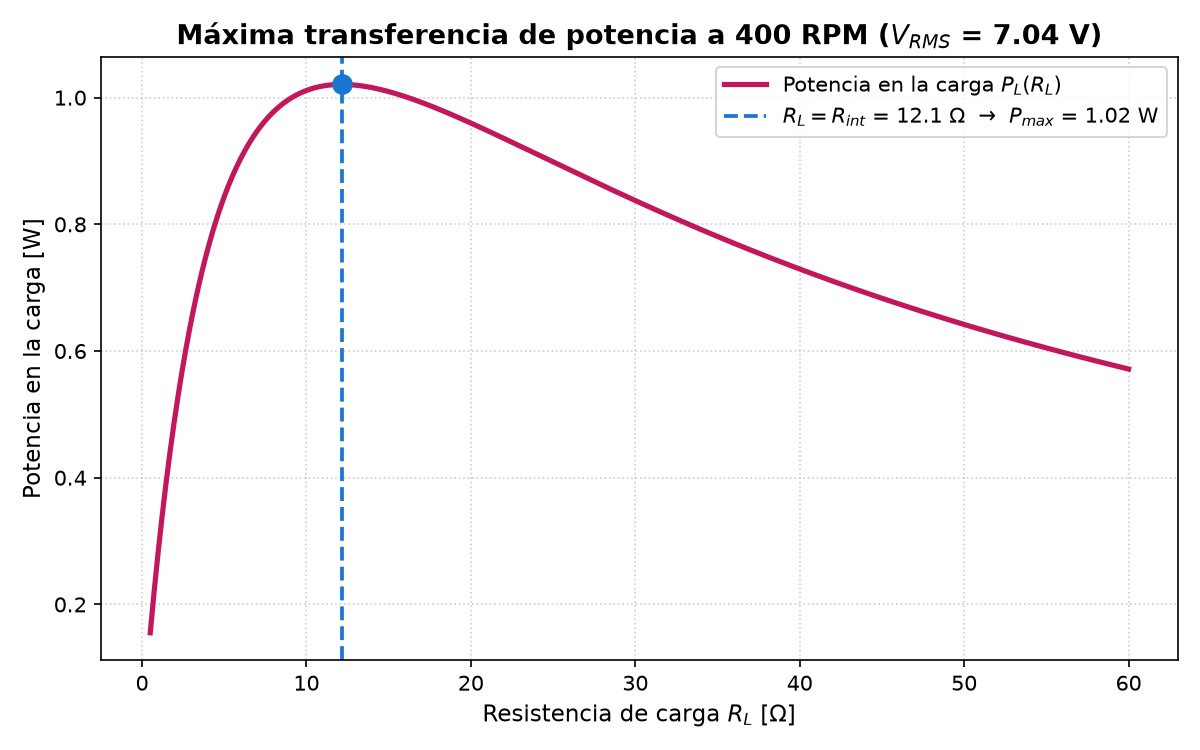
\includegraphics[width=0.8\linewidth]{04_potencia_vs_resistencia_carga.png}
\caption{Potencia en la carga en función de $R_L$: el máximo está exactamente en $R_L=R_{int}$.}
\end{figure}

\begin{figure}[H]
\centering
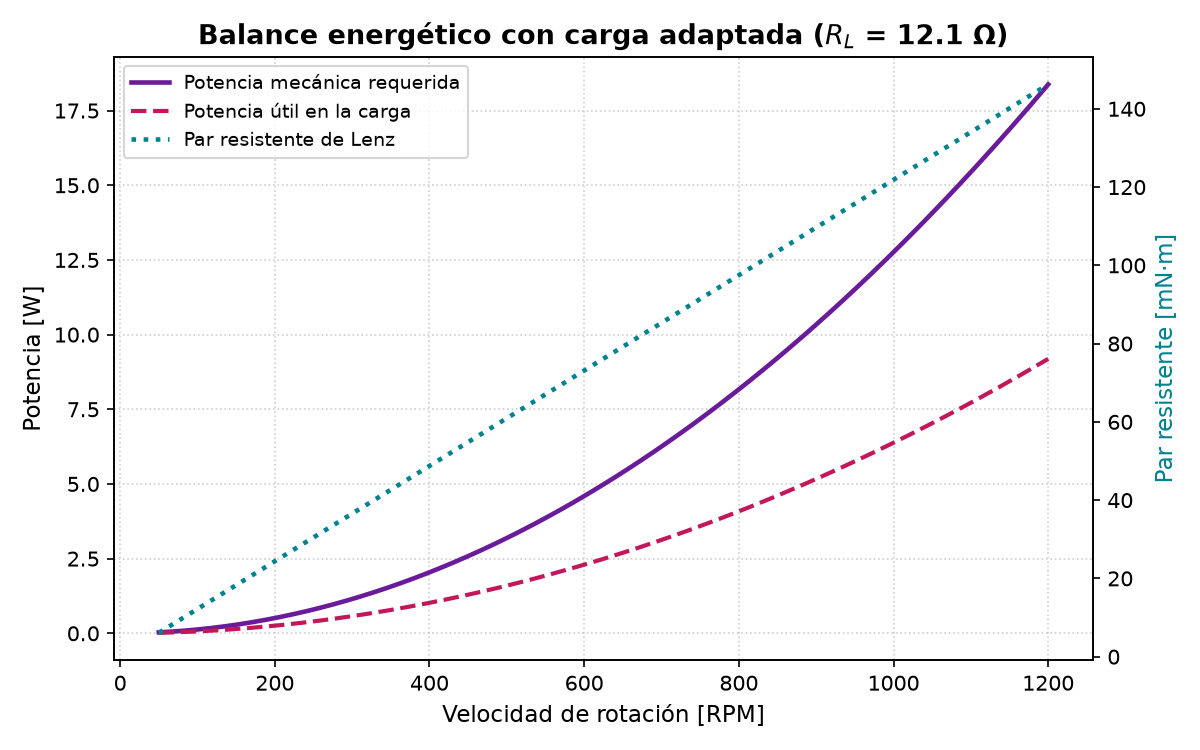
\includegraphics[width=0.8\linewidth]{05_potencia_y_par_lenz_vs_rpm.png}
\caption{Con carga adaptada la potencia crece con el cuadrado de la velocidad ($P\propto V^2\propto\text{RPM}^2$) y el
par resistente crece linealmente ($\tau=P/\omega_m\propto\text{RPM}$).}
\end{figure}

%=====================================================================
\section{Verificación de la etapa de salida}
%=====================================================================
\begin{paso}{Paso 13 · Condensador, LED y rizado}
\begin{itemize}
  \item \textbf{Tensión máxima} a \ValRpmMaxima\ RPM: $V_{DC}=\ValTensionDcMaxima$ V. El condensador de
        \ValTensionNominalCondensador\ V queda con un margen del \ValMargenCondensador\,\% (uno de 25\,V se dañaría).
  \item \textbf{LED} a \ValRpmMaxima\ RPM:
        $I_{LED}=\dfrac{V_{DC}-V_{LED}}{R_{LED}}=\dfrac{\ValTensionDcMaxima-\ValCaidaLed}{\ValResistenciaLed}=\ValCorrienteLedMaxMili$ mA
        (límite \ValCorrienteLedLimiteMili\ mA) y la resistencia disipa
        $I^2R=\ValPotenciaResistenciaLedMax$ W (nominal \ValPotenciaNominalResistenciaLed\ W).
  \item \textbf{Rizado} a \ValRpmReferencia\ RPM con el LED como carga ($I=\ValCorrienteLedRefMili$ mA):
        \[
          \Delta V_{pp}=\frac{I}{2f_eC}=\frac{\ValCorrienteLedRefMili\times10^{-3}}{2\times\ValFrecuenciaRef\times\ValCapacitanciaMicro\times10^{-6}}
          =\ValRizadoRef\ \text{mV}.
        \]
\end{itemize}
\end{paso}

%=====================================================================
\section{Micro-red a \ValRpmMicrored\ RPM}
%=====================================================================
\begin{paso}{Paso 14 · Batería (estado inicial SoC = \ValSocInicial\,\%)}
\begin{align*}
  E&=V_{nom}\,C=\ValBateriaTension\ \text{V}\times\ValBateriaCapacidad\ \text{Ah}=\ValBateriaEnergia\ \text{Wh},\\
  E_{oc}&=\ValBateriaVacia+\ValBateriaPendiente\times0.\ValSocInicial=\ValTensionOcRef\ \text{V},\\
  E_{util}&=(\text{SoC}-\text{SoC}_{corte})\,E=(0.\ValSocInicial-0.\ValSocCorte)\times\ValBateriaEnergia=\ValEnergiaUtilRef\ \text{Wh}.
\end{align*}
El inversor se desconecta al \ValSocCorte\,\% y vuelve a conectarse al \ValSocReconexion\,\%.
\end{paso}

\begin{paso}{Paso 15 · Carga con seguimiento del punto de máxima potencia}
\begin{align*}
  V_{RMS}&=\ValFemRmsMicrored\ \text{V},\qquad V_{DC}=\ValTensionDcMicrored\ \text{V}>\ValControladorArranque\ \text{V (arranca)},\\
  P_{max}&=\frac{V_{RMS}^2}{4R_{int}}=\frac{\ValFemRmsMicrored^2}{4\times\ValResistenciaInterna}=\ValPotenciaExtraibleMicrored\ \text{W},\\
  P_{bat}&=\eta_c\,P_{max}=0.\ValControladorEficiencia\times\ValPotenciaExtraibleMicrored=\boxed{\ValPotenciaHaciaBateria\ \text{W}},\\
  I_{carga}&=\frac{P_{bat}}{E_{oc}}=\frac{\ValPotenciaHaciaBateria}{\ValTensionOcRef}=\ValCorrienteCargaMicroredMili\ \text{mA}
  \quad(<\ValControladorCorrienteMax\ \text{A, no se limita}),\\
  P_{mec}&=P_{max}+I^2R_{int}=\ValPotenciaMecanicaMicrored\ \text{W},\qquad
  \tau=\ValParMicroredMili\ \text{mN}\cdot\text{m}.
\end{align*}
Sin consumo, recargar del \ValSocInicial\,\% al 100\,\% tomaría
$(1-0.\ValSocInicial)\times\ValBateriaCapacidad/0.\ValCorrienteCargaMicroredMili\approx\ValHorasRecarga$\,h.
\end{paso}

\begin{paso}{Paso 16 · Inversor de \ValInversorTension\,V / \ValInversorTensionAlta\,V a \ValInversorFrecuencia\,Hz}
\begin{align*}
  V_{pico}&=\sqrt2\times\ValInversorTension=\ValInversorPico\ \text{V}\qquad
  (\sqrt2\times\ValInversorTensionAlta=\ValInversorPicoAlto\ \text{V}),\\
  \frac{N_2}{N_1}&\approx\frac{\ValInversorPico}{\ValBateriaTension}=\ValRelacionEspiras,\\
  I_{AC}&=\frac{P_{AC}}{V_{RMS}}=\frac{\ValPotenciaCargaAc}{\ValInversorTension}=\ValCorrienteAcMili\ \text{mA},\\
  P_{in}&=\frac{P_{AC}}{\eta_{inv}}=\frac{\ValPotenciaCargaAc}{0.\ValInversorEficiencia}=\ValPotenciaEntradaInversor\ \text{W},\qquad
  I_{descarga}=\frac{P_{in}}{E_{oc}}=\ValCorrienteInversorBateria\ \text{A}.
\end{align*}
La potencia de \ValPotenciaCargaAc\,W está muy por debajo de la nominal del inversor (\ValInversorNominal\,W).
\end{paso}

\begin{paso}{Paso 17 · Balance de la batería y autonomía}
\begin{align*}
  P_{neta}&=P_{bat}-P_{in}=\ValPotenciaHaciaBateria-\ValPotenciaEntradaInversor=\boxed{\ValPotenciaNetaBateria\ \text{W}},\\
  t_{auto}&\approx\frac{E_{util}}{|P_{neta}|}=\ValAutonomiaHoras\ \text{h}\quad
  (\ValAutonomiaParadoHoras\ \text{h con el generador parado}).
\end{align*}
\end{paso}

\begin{paso}{Paso 18 · Velocidad de equilibrio}
Como $P_{bat}\propto\text{RPM}^2$, la velocidad que anula $P_{neta}$ para \ValPotenciaCargaAc\,W es
\[
  \text{RPM}_{eq}=\ValRpmMicrored\sqrt{\frac{\ValPotenciaEntradaInversor}{\ValPotenciaHaciaBateria}}\approx\ValRpmEquilibrio\ \text{RPM}.
\]
Supera las \ValRpmMaxima\ RPM del prototipo: \textbf{con \ValPotenciaCargaAc\,W la batería siempre se descarga}.
Con \ValPotenciaCargaReducida\,W el equilibrio se alcanza a $\approx\ValRpmEquilibrioReducida$\,RPM.
\end{paso}

\begin{figure}[H]
\centering
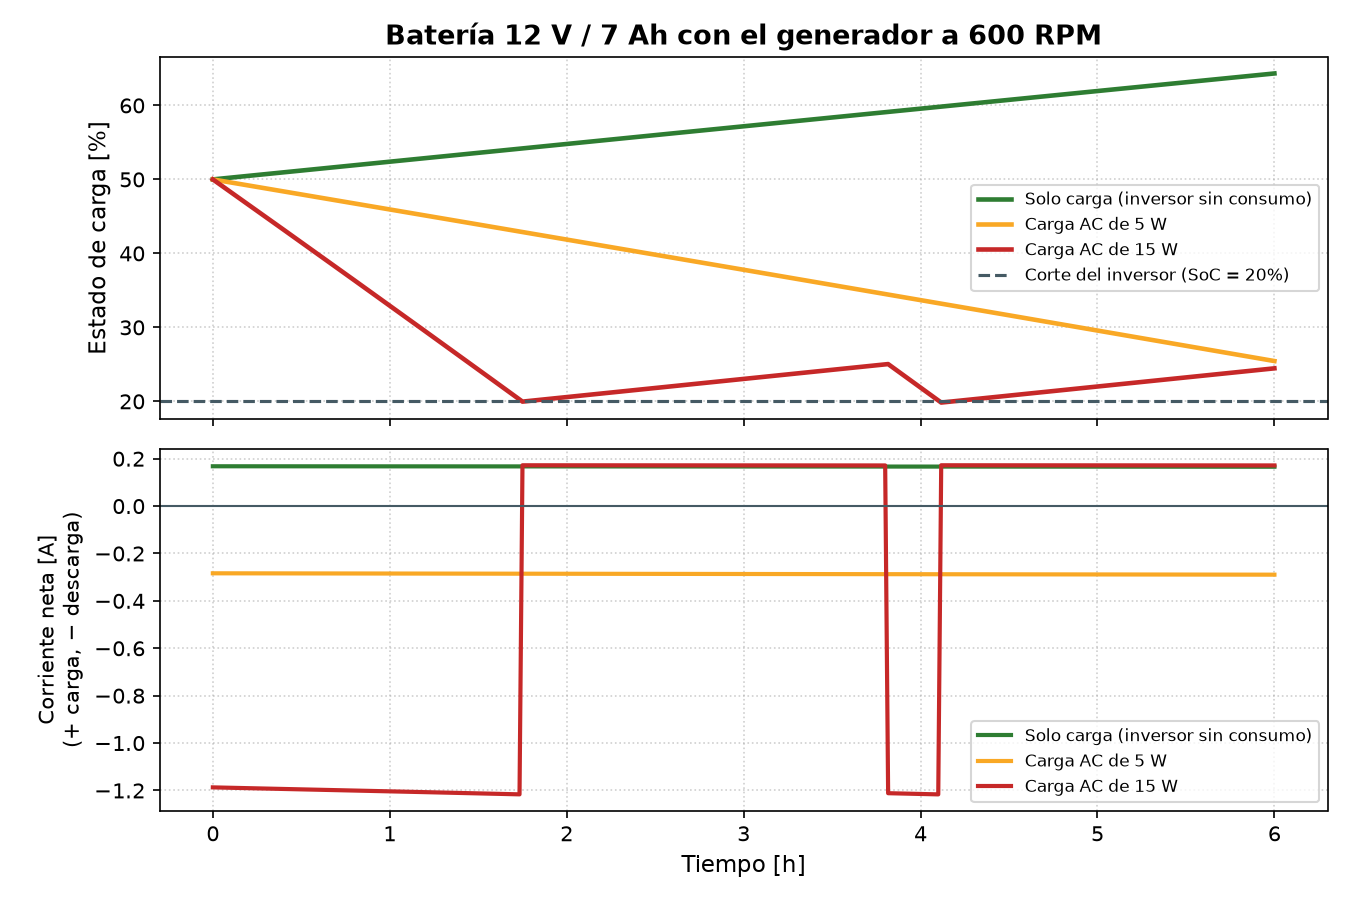
\includegraphics[width=0.85\linewidth]{06_curva_carga_bateria.png}
\caption{Evolución del SoC y de la corriente neta durante 6\,h a \ValRpmMicrored\ RPM con cargas de 0, 5 y 15\,W.
La línea discontinua marca el corte del inversor.}
\end{figure}

\begin{figure}[H]
\centering
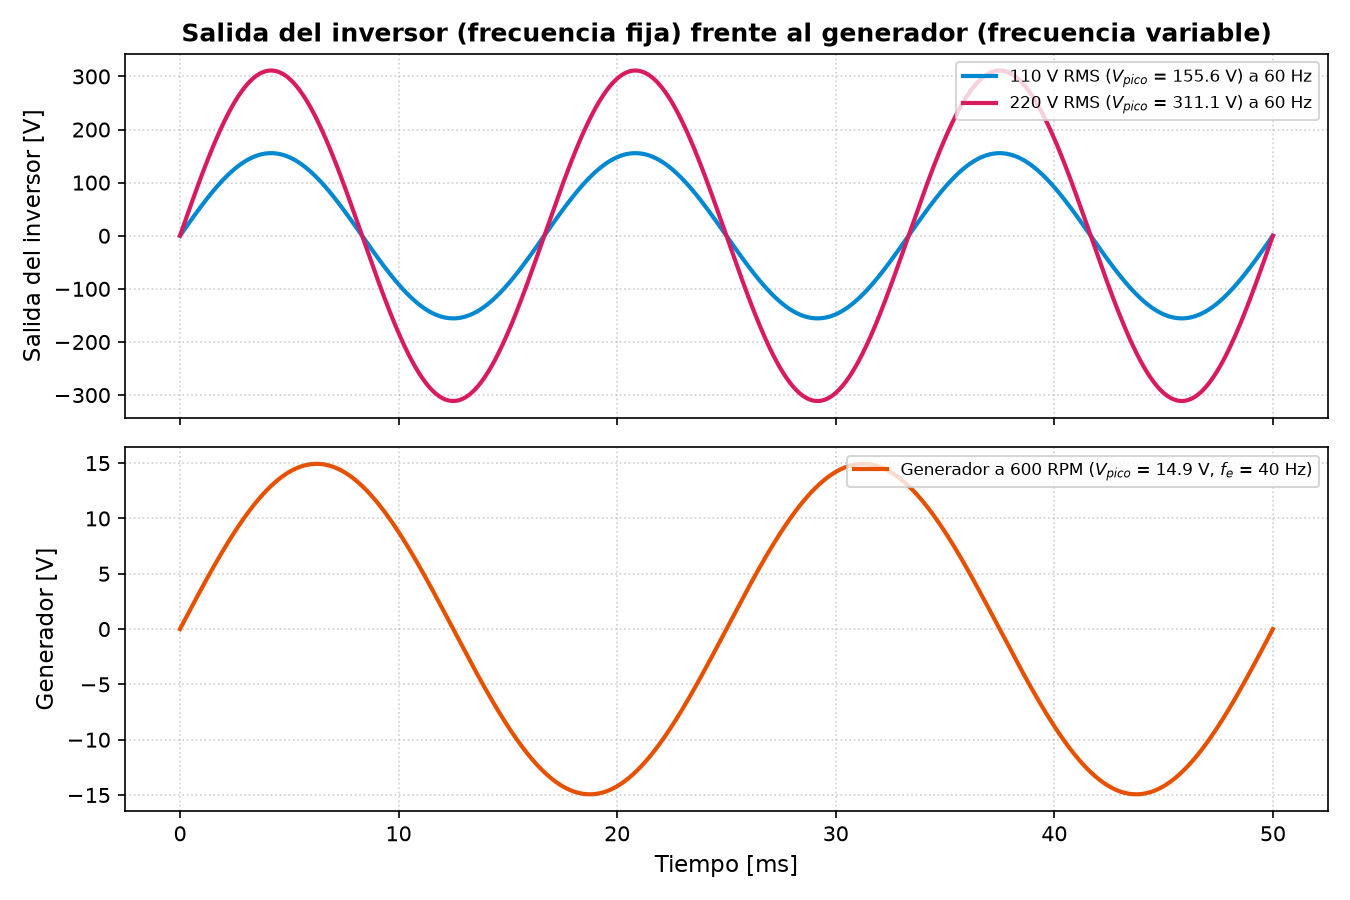
\includegraphics[width=0.85\linewidth]{07_onda_inversor_110v_220v.png}
\caption{Tensión del generador a \ValRpmMicrored\ RPM frente a la salida del inversor a 110\,V y 220\,V.}
\end{figure}

\begin{figure}[H]
\centering
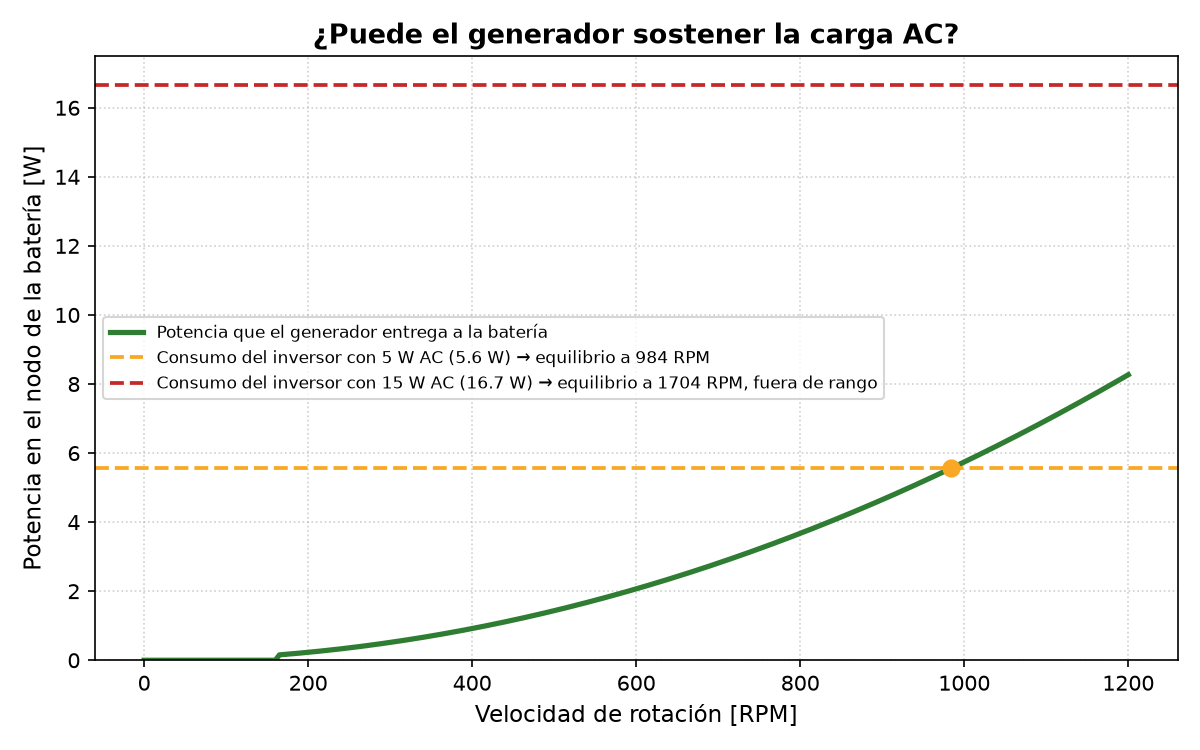
\includegraphics[width=0.85\linewidth]{08_balance_potencia_vs_rpm.png}
\caption{Potencia que llega a la batería frente al consumo del inversor. Los cruces son las velocidades de
equilibrio.}
\end{figure}

%=====================================================================
\section{Tabla de ensayos prevista}
%=====================================================================
\begin{table}[H]
\centering
\caption{Valores teóricos para el protocolo de pruebas (columnas en blanco: medidas del laboratorio).}
\small
\begin{tabular}{ccccccccc}
\toprule
Ensayo & RPM & $f_e$ [Hz] & $V_{pico}$ [V] & $V_{RMS}$ [V] & $V_{DC}$ [V] & $V_{RMS}$ med. & $V_{DC}$ med. & LED\\
\midrule
\filasdesde{generado/tabla_ensayos.tex}
\bottomrule
\end{tabular}
\end{table}

%=====================================================================
\section{Verificación automática del modelo}
%=====================================================================
El paquete de pruebas (\archivo{uv run pytest}) comprueba en cada cambio que:
\begin{enumerate}
  \item $B_z(0)$ coincide con $\frac{B_r}{2}\frac{L}{\sqrt{L^2+R^2}}$ y que a gran distancia el campo coincide con el de un
        dipolo equivalente (error menor al 0.1\,\%).
  \item El promedio analítico $\bar B_z$ coincide con una integración numérica de 20\,001 puntos (error relativo
        $<10^{-8}$).
  \item La fem calculada coincide con $-N_{total}\,\dif\Phi/\dif t$ obtenida por derivación numérica.
  \item La potencia máxima aparece en $R_L=R_{int}$ y se cumple $\tau\,\omega_m=P_L+P_{Cu}$.
  \item La salida DC no supera el 80\,\% de la tensión del condensador ni la potencia de la resistencia del LED.
  \item Las piezas STL son sólidos cerrados cuyo volumen coincide con el analítico (error menor al 0.5\,\%).
  \item La micro-red conserva la energía, respeta los límites del controlador, corta el inversor al \ValSocCorte\,\% y reconecta al \ValSocReconexion\,\%.
  \item El visualizador web (JavaScript) da exactamente los mismos resultados que Python.
\end{enumerate}

\end{document}
